\chapter{Technical Implementation}
This chapter delves into the practical realization of the CardioSync framework, translating the architectural concepts and design discussed in the previous chapters into tangible code and functional components. This chapter aims to offer an in-depth explanation of the coding process, including flowcharts and pseudo-code representations, showcasing how the theoretical foundation transforms into a working system.

\section{Hardware and Software Setup}
The implementation of the CardioSync framework involves both hardware and software components. This section outlines the necessary hardware setup and software environment required for the realization of the framework.

\subsection{Hardware Setup}
The CardioSync framework is built upon the FreeBie model, integrating the MAX30102 sensor. The hardware setup comprises the following components:

\begin{itemize}
    \item \textbf{FreeBie Mote:} This custom board in \autoref{fig:freebie} incorporates essential components, including the nRF52840 ARM-Based MCU module (\textit{EYSKBNZWB}) with BLE radio support, the External RTC and power management module (\textit{AB1815}), and FRAM (\textit{MB85RS4MT}). These components provide the foundation for the framework's intermittent operation.
    
    \item \textbf{MAX30102 Sensor Board:} The MAX30102 sensor board from Maxim Integrated serves as a critical element for heart rate monitoring. The sensor board features built-in pull-up resistors of 4.7k\(\Omega\) in the \(I^2C\) pin outs. However, for our specific use case, these resistors were not used, as the on-board pull up resistors of the nRF52840 were employed instead through Software configuration.
    
    \item \textbf{Connection Configuration:} Based on the pinout configuration of the FreeBie schematics, GPIO pin P0.04 is connected to the SCL (Serial Clock Line) of the MAX30102, while GPIO pin P0.27 is connected to the SDA (Serial Data Line). The MAX30102 is powered by the onboard super capacitors, connected to the \(V_{Batt}\) pinout of the FreeBie Mote.
\end{itemize}


\begin{figure}[H]
    \centering
    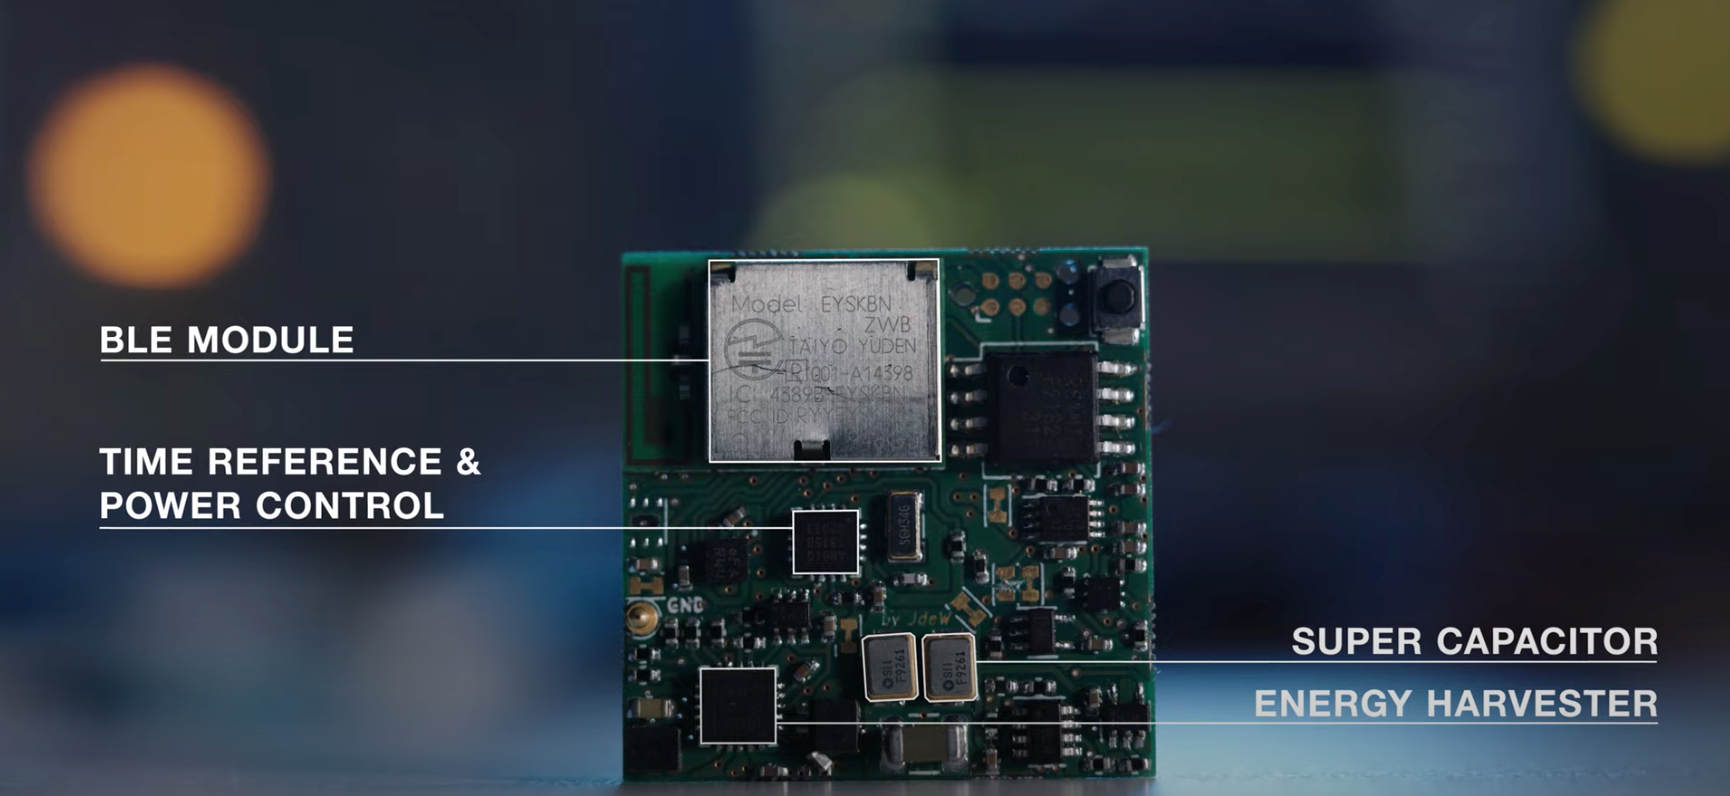
\includegraphics[width=\linewidth]{chapters/Implementation/Freebie.png}
    \caption{FreeBie Mote}
    \label{fig:freebie}
\end{figure}

\subsection{Software Setup}
\label{sec:software_setup_impl}

The implementation of the CardioSync framework builds upon the open-source FreeBie source code, available from the TUDelft Sustainable Systems Lab repository. The adaptation process involves customizing the existing \textit{"template"} application to accommodate the CardioSync system architecture  - MAX30102 sensor and the Heart Rate peak detection algorithm.

\subsubsection{Software Foundation and Customisation}

The entire FreeBie source code relies on the PacketCraft BLE stack, which seamlessly integrates nRF5 SDK libraries for driver interfaces and peripheral interactions. The code is specifically tailored for the nRF52840 MCU, utilizing the GNU ARM Embedded ToolChain, thus eliminating the need for additional build support or toolchain.

\subsubsection{MAX30102 Sensor Interfacing}

For interfacing with the MAX30102 sensor, nRFx driver for the Two Wire Interface - Master (TWIM) is employed. This involves enabling the necessary configurations in the \textit{sdk\_config.h} file to activate the TWIM in the system. Subsequently, relevant APIs provided by the nRFx library are utilized for reading from and writing to the \(I^2C\) interface.
 
\subsubsection{BLE Stack Configuration}

In the context of the BLE stack, PacketCraft's CMake configurations take charge of initializing the MCU as either a Peripheral or Central device. Two specific CMake definitions, namely \texttt{INIT\_PERIPHERAL} and \texttt{INIT\_CENTRAL}, determine the operational mode. PacketCraft then leverages essential components like the \textit{Device Manager (DM) and the Application framework main module (App)} to initialize the BLE stack. This equips the framework with APIs that helps with the initiation and termination of advertising or scanning activities depending on whether the device is operating as a Peripheral or Central.

\subsubsection{Timing and Scheduling}

Both the FreeBie and CardioSync frameworks require precise timing and scheduling mechanisms. PacketCraft's Wireless Software Foundation (WSF) OS layer offers essential APIs for managing the AppTimer functionality. These APIs enable the start and stop of timers, ensuring accurate timing operations necessary for the effective functioning of both frameworks.


\section{MAX30102 Sensor Interfacing}
Integral to the CardioSync framework is the seamless integration and interfacing with the MAX30102 sensor via the \(I^2C\) interface. This section delves into the practical implementation and methodologies used, outlining the steps taken to interface the MAX30102 sensor with the FreeBie architecture effectively.

\noindent As outlined in the previous section (\autoref{sec:software_setup_impl}), the existing "template" application within the FreeBie source code is extended to incorporate the MAX30102 sensor functionality. This is achieved by introducing a new source file named "\texttt{MAX30102\_main.c}", which houses all the necessary functions, declarations, and configurations essential for successful sensor interfacing and data acquisition.

\noindent The interfacing with the MAX30102 sensor involves several key functions, including sensor initialization, configuration setup, and data acquisition. Here is an in-depth look at these steps:

\subsection{Sensor Initialization and Configuration}
\label{sec:sensor_config}
The initialization of the MAX30102 sensor involves configuring its various registers to ensure optimal performance while minimizing power consumption. To achieve this, the \texttt{MAX30102\_init()} function is implemented. Within this function, several critical registers are configured as follows:

\begin{itemize}
    \item \textbf{REG\_INTR\_ENABLE\_1 (0x02U):} This register is set with the value 0xC0 to enable the "A\_FULL\_EN" interrupt, which triggers when the FIFO is full and data is ready for reading.
    
    \item \textbf{REG\_FIFO\_CONFIG (0x08U):} The FIFO configuration register is set with settings such as averaging 4 samples per entry, setting FIFO size to 32 (which triggers Interrupt 1 when full), and disabling FIFO rollover.
    
    \item \textbf{REG\_MODE\_CONFIG (0x09U):} Configures the operational mode of the sensor. In the context of CardioSync, heart rate mode is selected while disabling Spo2 measurements.
    
    \item \textbf{REG\_SPO2\_CONFIG (0x0AU):} Sets parameters for data acquisition including a sampling rate of 50 samples per second, ADC range of 4096nA, pulse width of 118us, and 16-bit ADC resolution.
    
    \item \textbf{REG\_LED1\_PA(0x0CU), REG\_LED2\_PA (0x0DU):} Configures LED current; for CardioSync, 1mA is set for both LED1 and LED2.
\end{itemize}

\noindent By meticulously configuring these registers, the MAX30102 sensor is primed to operate within desired parameters and less power consumption, yet capturing accurate blood flow data for heart rate analysis.

\subsection{Data Acquisition}
\label{sec:sensor_data_impl}
The data acquisition element of the MAX30102 sensor interfacing facilitates the collection of relevant sensor data to identify heart rate peaks. This section outlines the methodology employed for data collection, buffering, and sliding window management within the CardioSync framework.

\noindent A two dimensional buffer of a maximum capacity of 2 x 500 entries is employed to store the current sensor values and their respective RTC ticks at which they are read. These values are continuously read from the MAX30102 sensor's FIFO and \texttt{PalRtcCounterGet()} at a predetermined sampling rate. In parallel, a sliding window of size 10 is established, ensuring that the latest 10 sensor values are always maintained within the window.

\noindent The data acquisition process is orchestrated by the following key steps:

\subsubsection{WSF Timer Initialization}
Upon successful sensor initialization, a WSF timer named "\texttt{MAX30102Timer}" is initiated. The timer's period is determined by \(1000\) divided by the chosen sampling rate. In the context of the CardioSync architecture, a sampling rate of \(100\) Hz is selected after rigorous evaluation of both the sensor's capabilities and the heart rate peak detection algorithm. Further insights into the rationale behind this decision are provided in the upcoming "Results" chapter (\ref{chap:results}).

\subsubsection{FIFO Read and Buffering}
When the "\texttt{MAX30102Timer}" timer expires, it triggers an event labeled "MAX30102\_TIMER\_IND." Within the scope of this event, the MAX30102 sensor's FIFO is read using the "\texttt{MAX30102\_read\_fifo()}" function. This function relies on the \texttt{nrfx\_twim} module to extract the current IR and Red LED values from the FIFO. Among these values, the IR value holds samples for heart rate peak detection. Consequently, the IR value is paired with the corresponding RTC ticks recorded during the sensor read and appended to the end of the buffer.

\subsubsection{Continuous Data Acquisition}
Following the FIFO read and buffering, the "\texttt{MAX30102Timer}" is restarted. This sequence of operations repeats at intervals of \(10\) ms until the sliding window, positioned at the end of the buffer, is completely populated with the latest \(10\) values. This data acquisition process ensures that the sliding window is consistently updated, offering a continuous stream of data for subsequent heart rate peak detection.

\subsubsection{Heart Rate Peak Detection}
The sensor values contained within the sliding window are then subjected to the heart rate peak detection algorithm only if the average of those 10 values in Sliding window more than 8000. Peak detection is conducted only when the sensor comes into contact with a person. In the absence of such contact, the average value is expected to be below 8000. This algorithm is designed to identify peaks indicative of heart rate activity, allowing the CardioSync framework to accurately determine heart rate patterns based on the IR values.

\noindent The iterative nature of this process guarantees the availability of up-to-date sensor data for real-time heart rate analysis, ensuring the responsiveness and accuracy of the CardioSync system.

\subsubsection{Pseudocode Representation}
For better understanding, here is a pseudocode representation of the data acquisition process:

\begin{algorithm}[H]
\caption{MAX30102 Sensor Data Acquisition}
\begin{algorithmic}[1]

\State Initialize 2D Buffer with maximum capacity of 2 x 500
\State Initialize Sliding Window size as 10
\State Initialize "\textit{\texttt{MAX30102Timer}}" with period \(1000 / Sampling\ Rate\)
\State Start "\textit{\texttt{MAX30102Timer}}"

\State Wait for "\textit{\texttt{MAX30102Timer}}" to expire
\If{\textit{\texttt{MAX30102Timer}} expired}
    \State Read MAX30102 sensor's FIFO using "MAX30102\_read\_fifo()"
    \State Append IR value and corresponding RTC ticks to Buffer
    \If{Sliding Window is full and Average > 8000}
        \State Perform Heart Rate Peak Detection on Sliding Window data
    \EndIf
    \State Restart "\textit{\texttt{MAX30102Timer}}"
\EndIf

\end{algorithmic}
\end{algorithm}

\subsection{Heart Rate Peak Detection Algorithm}
\label{sec:heart_rate_algo_impl}
Initially, an attempt was made to utilize Maxim Integrated's heart rate peak detection algorithm developed for MAXREFDES117. This algorithm employed a method of peak identification by calculating a fixed threshold and detecting peaks above that threshold. Additionally, it employed a fixed threshold for removing closely spaced peaks based on a parameter \(n_{min\_distance}\). However, this approach proved ineffective for the CardioSync framework due to the dynamic and varying nature of the continuous sensor data readings obtained from the MAX30102. As shown in Figure~\ref{fig:dynamic_threshold}, the sensor data exhibited fluctuations that necessitated a more adaptive and dynamic thresholding approach.

\begin{figure}[H]
    \centering
    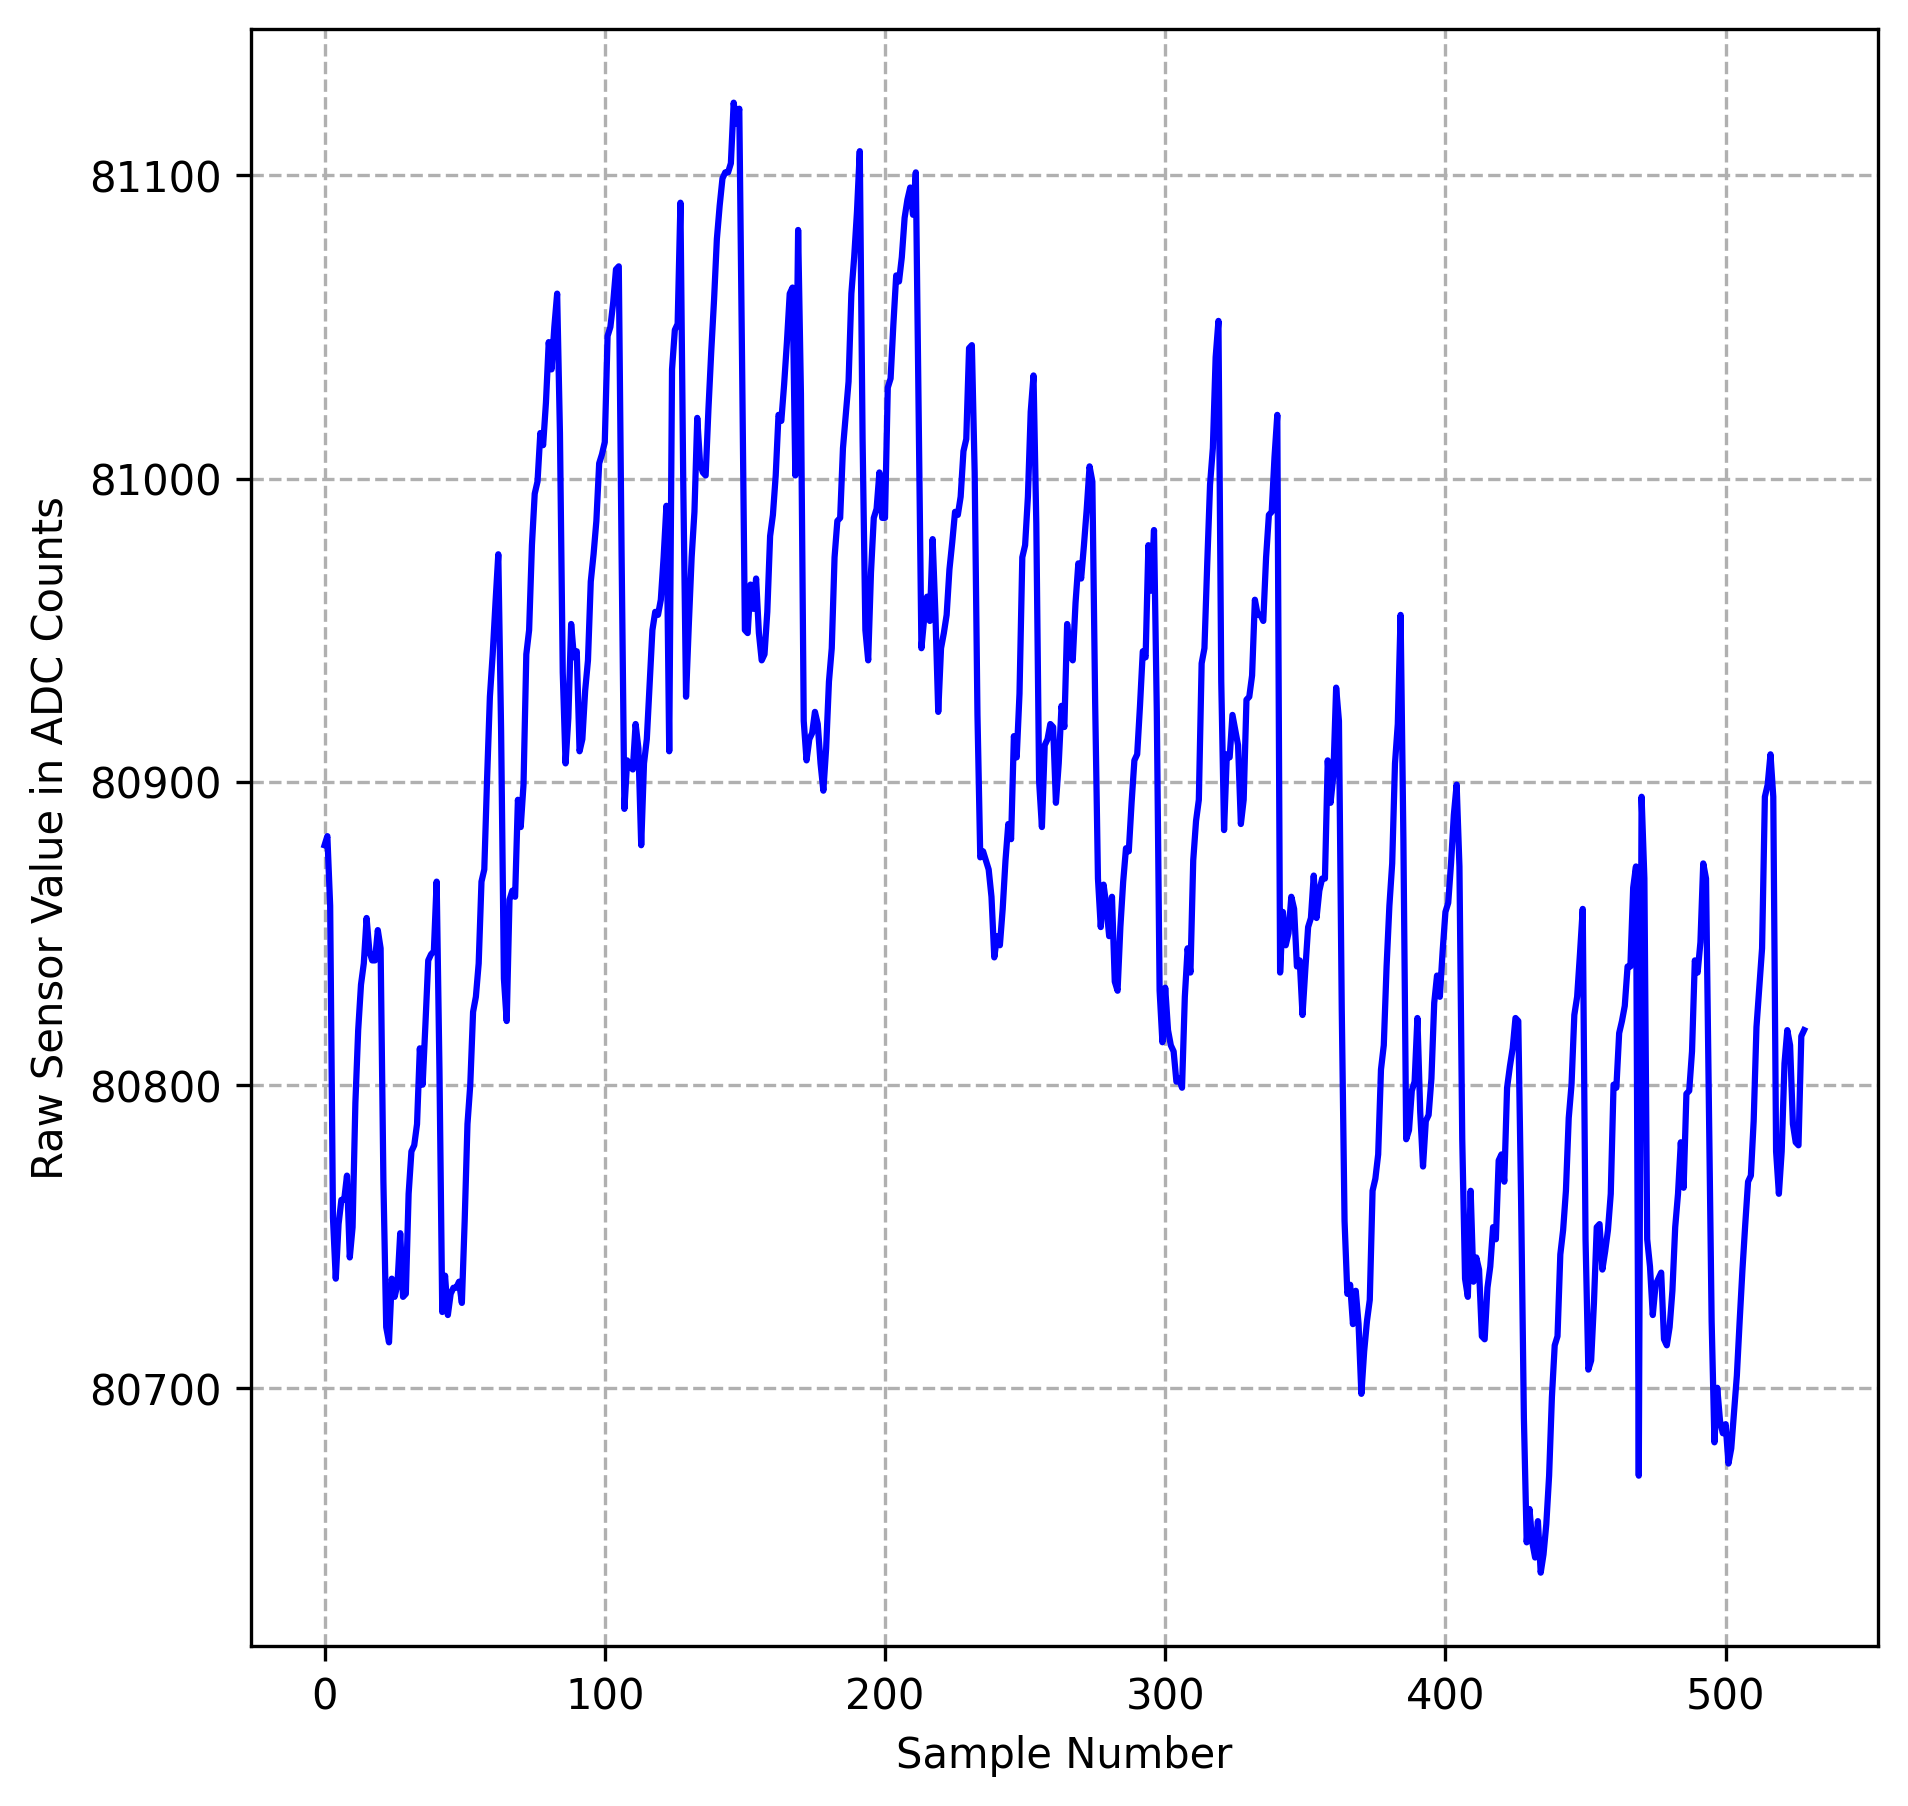
\includegraphics[width=0.7\linewidth]{chapters/Implementation/dynamic_threshold.png}
    \caption{Dynamic and fluctuating nature of continuous sensor data readings from MAX30102}
    \label{fig:dynamic_threshold}
\end{figure}

\noindent In light of these challenges, the decision was made to adopt an alternative approach that leverages the derivatives of the sensor data for peak detection. This approach was more suitable for handling the varying nature of the sensor readings and provided a robust means of detecting heart rate peaks.

\noindent The heart rate peak detection algorithm using derivatives operates as follows:

\begin{enumerate}
    \item \textbf{Data Preprocessing:} The raw sensor data collected from Sliding window buffer, denoted as \(a_{ir}\), undergoes preprocessing steps. The algorithm removes the DC component by calculating the mean and subtracting it from the data. This step is essential to eliminate any static offset and focus on the variations caused by heartbeats.
    
    \item \textbf{Moving Average:} The \(a_{ir}\) data is then updated using a moving average of two neighboring samples on either side of each sample. This smoothing technique helps reduce noise and sharp variations in the data, facilitating more accurate peak detection.
    
    \item \textbf{Derivative Calculation:} The first derivative of the \(a_{ir}\) data, referred to as \(a_{ir\_diff}\), is calculated. This derivative provides insights into the rate of change of the signal, which is particularly useful for identifying rapid transitions characteristic of heart rate peaks.
    
    \item \textbf{Peak and Valley Detection:} The algorithm identifies peaks and valleys within the \(a_{ir\_diff}\) data. Peaks correspond to points where the derivative changes from positive to negative, indicating a downward slope. Valleys, conversely, represent points where the derivative changes from negative to positive, indicating an upward slope. These points mark significant variations in the signal, which are indicative of heart rate peaks.
    
    \item \textbf{Peak Validation and Removal:} Detected peaks that are in close proximity to valley indices are discarded. A maximum distance threshold \(n_{valley\_distance}\) of value \textbf{4} is used to determine this proximity. Similarly, peaks that are too close to each other, within a distance threshold \(n_{peak\_distance}\) of value \textbf{15}, are also removed. These additional validation steps help ensure that the detected peaks correspond to distinct heart rate events.
    
    \item \textbf{Result Generation:} The algorithm generates a list of validated peak indices that represent heart rate peaks which likely to have occurred.
    
    \item \textbf{Callback and Post Processing:} For each detected and validated peak index, the algorithm invokes the \texttt{sensor\_callback} function. This function handles further processing, synchronization, and scheduling tasks related to the CardioSync framework.
\end{enumerate}

\noindent The constants \(n_{valley\_distance}\), and \(n_{peak\_distance}\) are empirically determined based on the characteristics of the sensor data and the expected heart rate patterns. These values ensure the reliability and accuracy of the peak detection process.

\noindent The algorithm's pseudocode is as follows:

\begin{algorithm}[H]
\caption{Heart Rate Peak Detection Algorithm - calculate\_heart\_rate}
\begin{algorithmic}[1]
\Function{calculate\_heart\_rate}{$a\_ir, callback$}
    \State Initialize arrays $a\_ir\_clean$, $a\_ir\_diff$, $peak\_indices$, and $valley\_indices$
    \State Calculate the mean of the raw IR sensor data $a\_ir$ to remove the DC component and obtain a centered signal
    
    \For{each data point $x$ in $a\_ir$}
        \State Subtract the mean from each data point to center the signal around zero, storing the result in $a\_ir\_clean$
    \EndFor
    
    \For{each data point $x$ in $a\_ir\_clean$}
        \State Apply a moving average filter to $a\_ir\_clean$ by averaging nearby two data points on both side to reduce noise and fluctuations
    \EndFor
    
    \For{each data point $x$ in $a\_ir\_clean$}
        \State Calculate the first derivative of the filtered signal $a\_ir\_clean$ to highlight changes in the signal, storing the result in $a\_ir\_diff$
    \EndFor

    \For{each index $x$ in the range from $1$ to $n - 2$, where $n$ is the length of $a\_ir\_diff$}
        \If{$a\_ir\_diff[x - 1]$ is positive \textbf{and} $a\_ir\_diff[x]$ is negative}
            \State Store the peak index $x$ in the $peak\_indices$ array
        \EndIf
    \EndFor

    \For{each index $x$ in the range from $1$ to $n - 2$, where $n$ is the length of $a\_ir\_diff$}
        \If{$a\_ir\_diff[x - 1]$ is negative \textbf{and} $a\_ir\_diff[x]$ is positive}
            \State Store the peak index $x$ in the $valley\_indices$ array
        \EndIf
    \EndFor
    
    \State Apply a post-processing step to remove peaks that are too close to each other using $n\_peak\_distance$
    % \For{each index $i$ in the range from $0$ to $peak\_indices\_length - 2$}
    %     \If{$peak\_indices[i + 1] - peak\_indices[i] < n\_peak\_distance$}
    %         \State Remove the peak at index $i + 1$ from $peak\_indices$
    %     \EndIf
    % \EndFor
    
    \State Apply a post-processing step to remove peaks that are close to valley indices using $n\_valley\_distance$
    % \For{each peak index $p$ in $peak\_indices$}
    %     \For{each valley index $v$ in $valley\_indices$}
    %         \If{$|p - v| < n\_valley\_distance$}
    %             \State Remove the peak at index $p$ from $peak\_indices$
    %         \EndIf
    %     \EndFor
    % \EndFor
    
    \State Call the callback function with the detected peak indices in $peak\_indices$
    
\EndFunction
\end{algorithmic}
\end{algorithm}

\noindent This algorithm's robustness and adaptability are crucial for accurately identifying heart rate peaks in the CardioSync framework, even when dealing with dynamic and fluctuating sensor data.

\section{Putting it Together}
With the fundamental components of the CardioSync framework established—ranging from hardware setup to heart rate peak detection algorithms, the next step involves integrating these elements into the FreeBie architecture. This section provides insight into how these various parts work together to create a functional system, ensuring accurate heart rate peak detection and synchronized BLE connection setup within a battery less system architecture.

\subsection{Framework Integration in the Template Application}
As previously mentioned in section \ref{sec:software_setup_impl}, the CardioSync framework is a part of the "\textit{template}" application in the FreeBie source code. Focusing from the start of execution, the MAX30102 sensor module is initialised through \texttt{MAX30102HandlerInit()} from within the application's stack init along with several required setup for BLE stack such as the \textit{Device Manager} and \textit{Application Manager}, \textit{Slave or Master initialization} according to the device's operational mode.

\noindent Within the \texttt{MAX30102HandlerInit()} function, \texttt{MAX30102\_config() and MAX30102\_init()} performs the configuration and activation of the TWIM interface for the MAX30102 sensor with  the parameters and operating configurations discussed in Section \ref{sec:sensor_config}. It's noteworthy that the MAX30102 is assigned to \textit{TWI instance 1}, as \textit{TWI instance 0} is exclusively allocated for SPI communication with the external FRAM module in the FreeBie architecture.

\subsection{WSF Timer Setup and Template Application Start}
The MAX30102HandlerInit function also initialises vital WSF timers \textit{MAX30102Timer} and \textit{MAX30102RestartTimer}. The comprehensive roles and functionalities of these timers will be elaborated upon in the subsequent sections. 

\noindent Upon the successful initiation of the system's BLE stack and the MAX30102 sensor, the "template" application commences its operation by invoking \texttt{TemplateStart()}. This phase encompasses the registration of BLE-related callbacks and attribute server setups. This sequence ends with a trigger of a Device Manager reset, setting the stage for subsequent phases.

\subsection{Sensor Data Acquisition and Peak Detection}
With the Device Manager reset, all essential initializations have been accomplished, paving the way for sensor data acquisition with the invocation of the \texttt{MAX30102Start()} function within the context of the "\texttt{DM\_RESET\_CMPL\_IND}" event handler in \texttt{TemplateHandler()}. It triggers buffer clearance and sliding window initialization. Followed by that, it starts the primary \textit{MAX30102Timer}, which orchestrates sensor data reading at a 100Hz sampling rate and facilitates heart rate peak detection. The details of these processes are elaborated in Sections \ref{sec:sensor_data_impl} and \ref{sec:heart_rate_algo_impl}.

\subsection{Heart Rate Peaks Post Processing and BLE Connection Initiation}
With the successful identification of heart rate peaks, their corresponding indices within sliding window are passed to the \texttt{sensor\_callback()} routine, marking the commencement of post-processing and synchronization tasks. This pivotal mechanism forms the CardioLink Synchronisation hub component embedded within the CardioSync framework architecture.

\noindent For each heart rate peak, the concomitant system RTC tick is retrieved from the data stored in a two-dimensional buffer using its indices.This paired data allows the \texttt{sensor\_callback()} function to distinguish between new peaks and peaks that linger within the rotating buffer. When a new peak is identified, the function updates the global variable \texttt{average\_time\_diff}, encapsulating the average time difference between the present peak and the previously detected peaks, i.e., heart rate interval. This value plays a pivotal role in establishing heart rate-based synchronization points.

\subsection{BLE Connection Setup and Synchronization}
Subsequently, based on the system's operational mode, either advertisement or scan initiation happens using PacketCraft's Application Manager API, such as \texttt{AppAdvStart()} or \texttt{AppScanStart()}. These operations are executed utilizing carefully optimized BLE parameters, encompassing advertising interval, scanning interval, scan duration, and scan window. These parameters are strategically chosen based on the comprehensive evaluation of algorithm performance and system behavior outlined in the forthcoming Results and Evaluation(\autoref{chap:results}) under the table \ref{tab:ble_params}. 

\noindent This phase operates simultaneously with active sensor read at a 100Hz sampling rate and synchronized advertising or scanning events correlated to each detected heart rate peak.

\subsection{Adaptive Heart Rate Recalculation and System Power Management}
Following the detection of three peaks (\texttt{MAX\_PEAKS}), \texttt{MAX30102Stop()} is invoked, shutting down the sensor by configuring the \texttt{REG\_MODE\_CONFIG} register (0x09U) with the value 0x80. This activates the MAX30102 Shutdown Control bit, facilitating power-saving mode in sensor. Simultaneously, the \texttt{MAX30102Timer} is terminated, suspending active sensor read.

\noindent After this phase, BLE parameters are dynamically adjusted during runtime to ensure the scheduling of advertisement or scanning events aligned with the heart rate interval. This adjustment relies on the \texttt{average\_time\_diff} global variable, which is continously updated during active sensor read and heart rate peak detection. The modified BLE parameters are outlined in Table \ref{tab:modified_ble_params}.

\begin{table}[H]
\centering
\begin{tabular}{|cc|}
\hline
\multicolumn{2}{|c|}{\textbf{\begin{tabular}[c]{@{}c@{}}BLE Advertisement Parameters\\ (Peripheral)\end{tabular}}} \\ \hline
\multicolumn{1}{|c|}{\textit{Advertising Interval}} & Heart rate interval \\ \hline
\multicolumn{1}{|c|}{\textit{Advertising Duration}} & 10 seconds          \\ \hline
\multicolumn{2}{|c|}{\textbf{\begin{tabular}[c]{@{}c@{}}BLE Scan Parameters\\ (Central)\end{tabular}}}             \\ \hline
\multicolumn{1}{|c|}{\textit{Scan Interval}}        & Heart rate interval \\ \hline
\multicolumn{1}{|c|}{\textit{Scan Window}}          & 100 milliseconds    \\ \hline
\multicolumn{1}{|c|}{\textit{Scan Duration}}        & 10 seconds          \\ \hline
\end{tabular}
\caption{Modified BLE parameters during runtime based on calculated heart rate interval (\texttt{average\_time\_diff})}
\label{tab:modified_ble_params}
\end{table}

\noindent This sets the stage for real-time task scheduling through APIs like \texttt{AppAdvStart()} or \texttt{AppScanStart()} using modified BLE parameters, engaging the Checkpointing and Restore module embedded within the FreeBie architecture. It detects for inactivity in the system, here in our case it is caused by no active sensor reads, and then initiates the process that checkpoints the current state of system and proceeds to power down the microcontroller unit (MCU), thereby placing it into a sleep mode. The system resumes and restores its operations only during planned BLE connection events, then returning to a sleep state until the subsequent heart rate interval. The current phase of the BLE connection setup process relies on the synchronization point established through the heart rate interval. It aims to conserve power by adhering to the principles of the FreeBie architecture. This approach enables synchronized advertisement or scanning, as opposed to periodic asynchronous methods, in order to establish a connection between two battery-less endpoints. 

\noindent In cases where connection establishment eludes success even during this phase, the continuity of heart rate interval (\texttt{average\_time\_diff} may be compromised. Thus, an adaptive approach comes into play. To address this, the \texttt{MAX30102RestartTimer} set for a 10-second duration, is activated in tandem with the scheduled BLE connection synchronization points when the \texttt{MAX\_PEAKS} has been detected. Upon the timer expiry, the sensor data buffers, previously detected peaks, and the \texttt{average\_time\_diff} global variable are reset. Subsequently, \texttt{MAX30102Start()} is invoked anew, reinitiating active sensor read. This iterative process continues until successful BLE connection is established. Upon connection close, \texttt{MAX30102Start()} is re-invoked, initiating the entire process afresh.


\noindent In summary, the implementation of the CardioSync framework within the FreeBie architecture constitutes a cohesive integration of hardware and software components. The collaboration between the MAX30102 sensor, heart rate peak detection algorithm, and BLE connection setup mechanisms underscores the system's ability to seamlessly detect heart rate peaks and synchronize BLE connections, all while adhering to the low-power principles of FreeBie architecture.

\noindent The operational flow of this process can be better understood through the comprehensive flowchart in \autoref{fig:flowchart}, that captures the interactions between the components at each stage. While this chapter has delved into the intricate details of implementation, the next chapter delves into the empirical evaluation of the system's performance, offering insights into the effectiveness and efficiency of the CardioSync framework.

\begin{figure}[H]
    \centering
    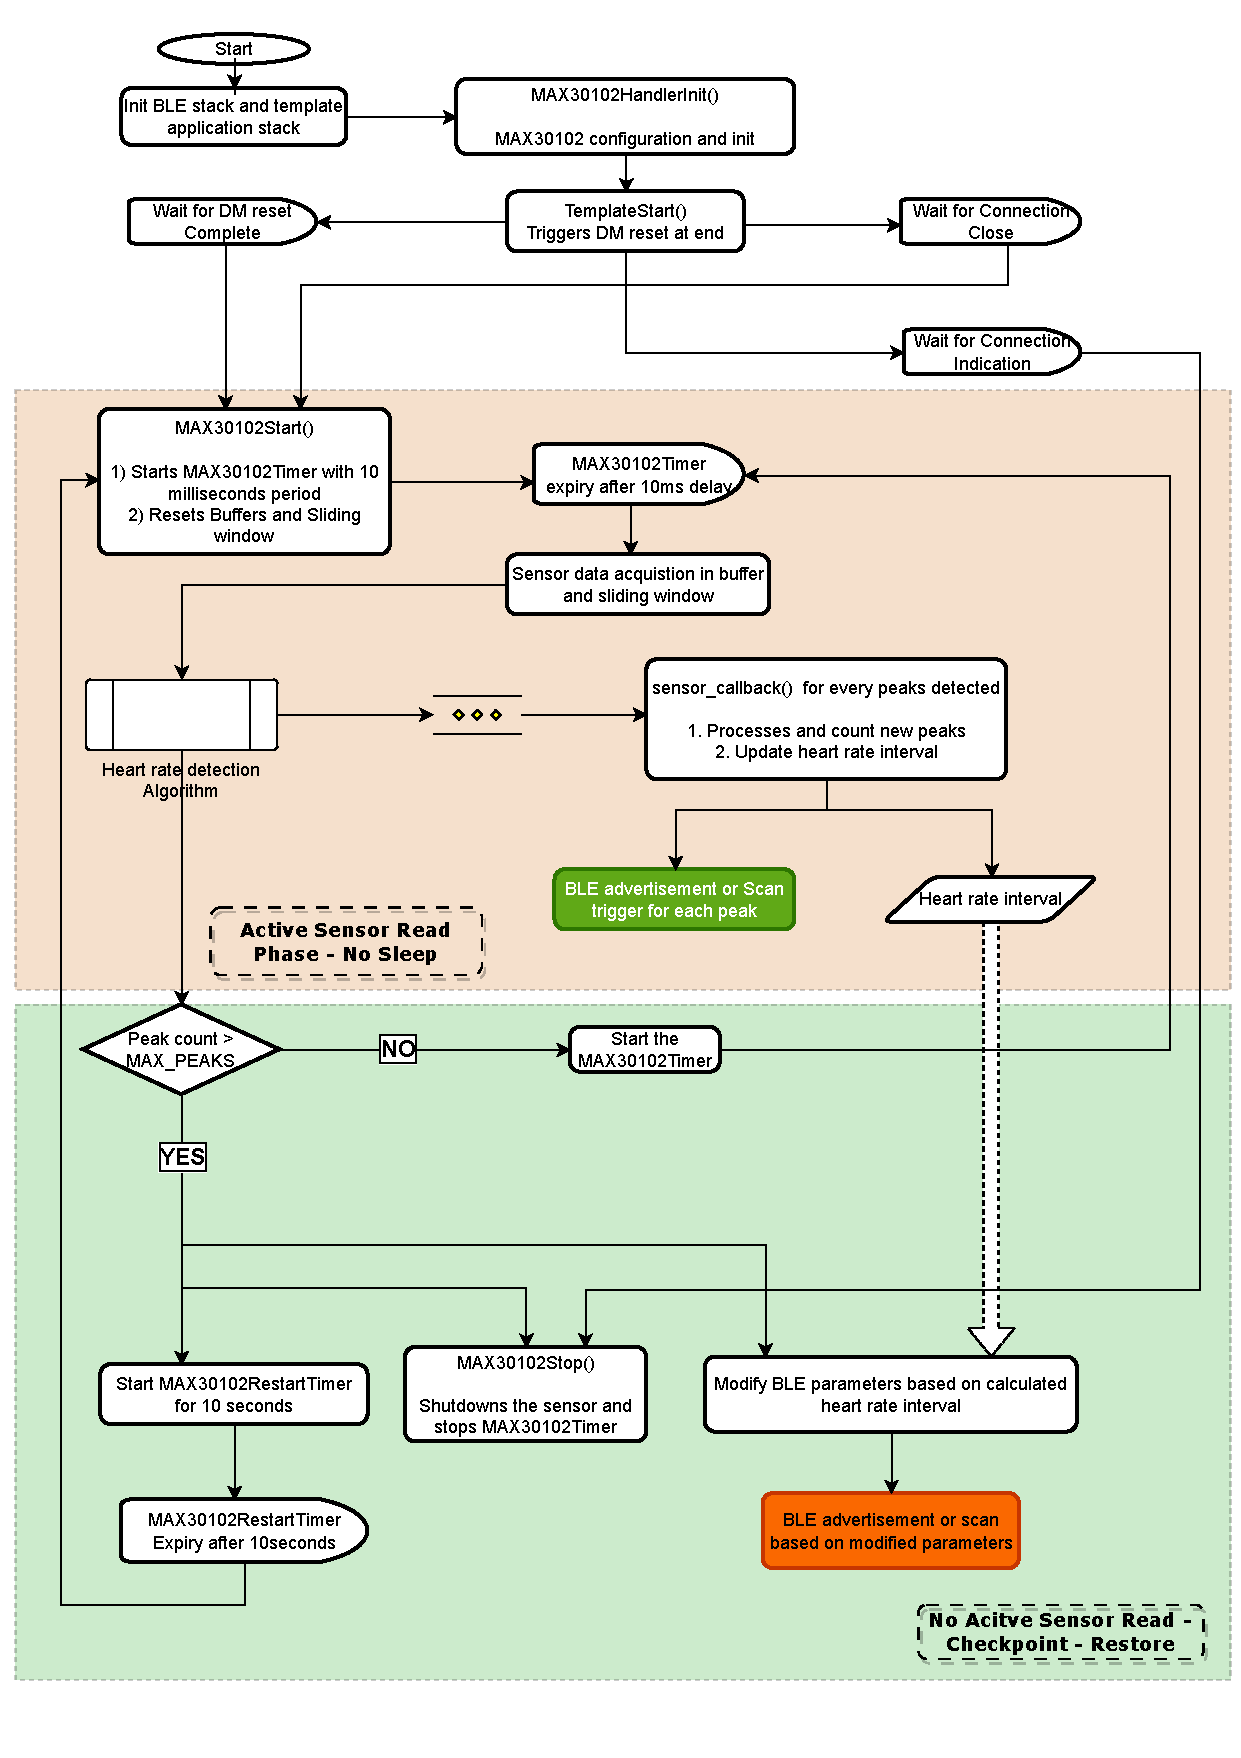
\includegraphics[width=\linewidth]{chapters/Implementation/Flowchart_CardioSync.pdf}
    \caption{Operation flowchart of the CardioSync framework implementation}
    \label{fig:flowchart}
\end{figure}